\chapter{Integration strategy}\label{chap:strategy}

\section{Entry criteria}
% Specify the criteria that must be met before integration testing of specific elements may begin (e.g., functions must have been unit tested).
The first obvious condition which needs to be satisfied before starting the integration test process is that the modules to be integrated are fully developed. 

Moreover,in order to provide a reliable background, most of the functions shall have already been unit tested. In detail, we require that at least \SI{75}{\percent} of each component to be integrated has been unit tested.\footnote{\color{red}ANDREA \`E RAGIONEVOLE?} 

It is also important that some mock data are created, in order to let the components work. Please, refer to \cref{chap:stubs} for further details.\footnote{\color{red}DEVO AGGIUNGERE ALTRO?}




\section{Elements to be integrated}
% Identify the components to be integrated, refer to your design document to identify such components in a way that is consistent with your design.
Integration testing deals with components. That is why in the following we are showing in \cref{fig:component} the component diagram of myTaxiService system, already presented in section~2.3 of the \emph{Design document}.

\begin{figure*}%
	\centering% 
	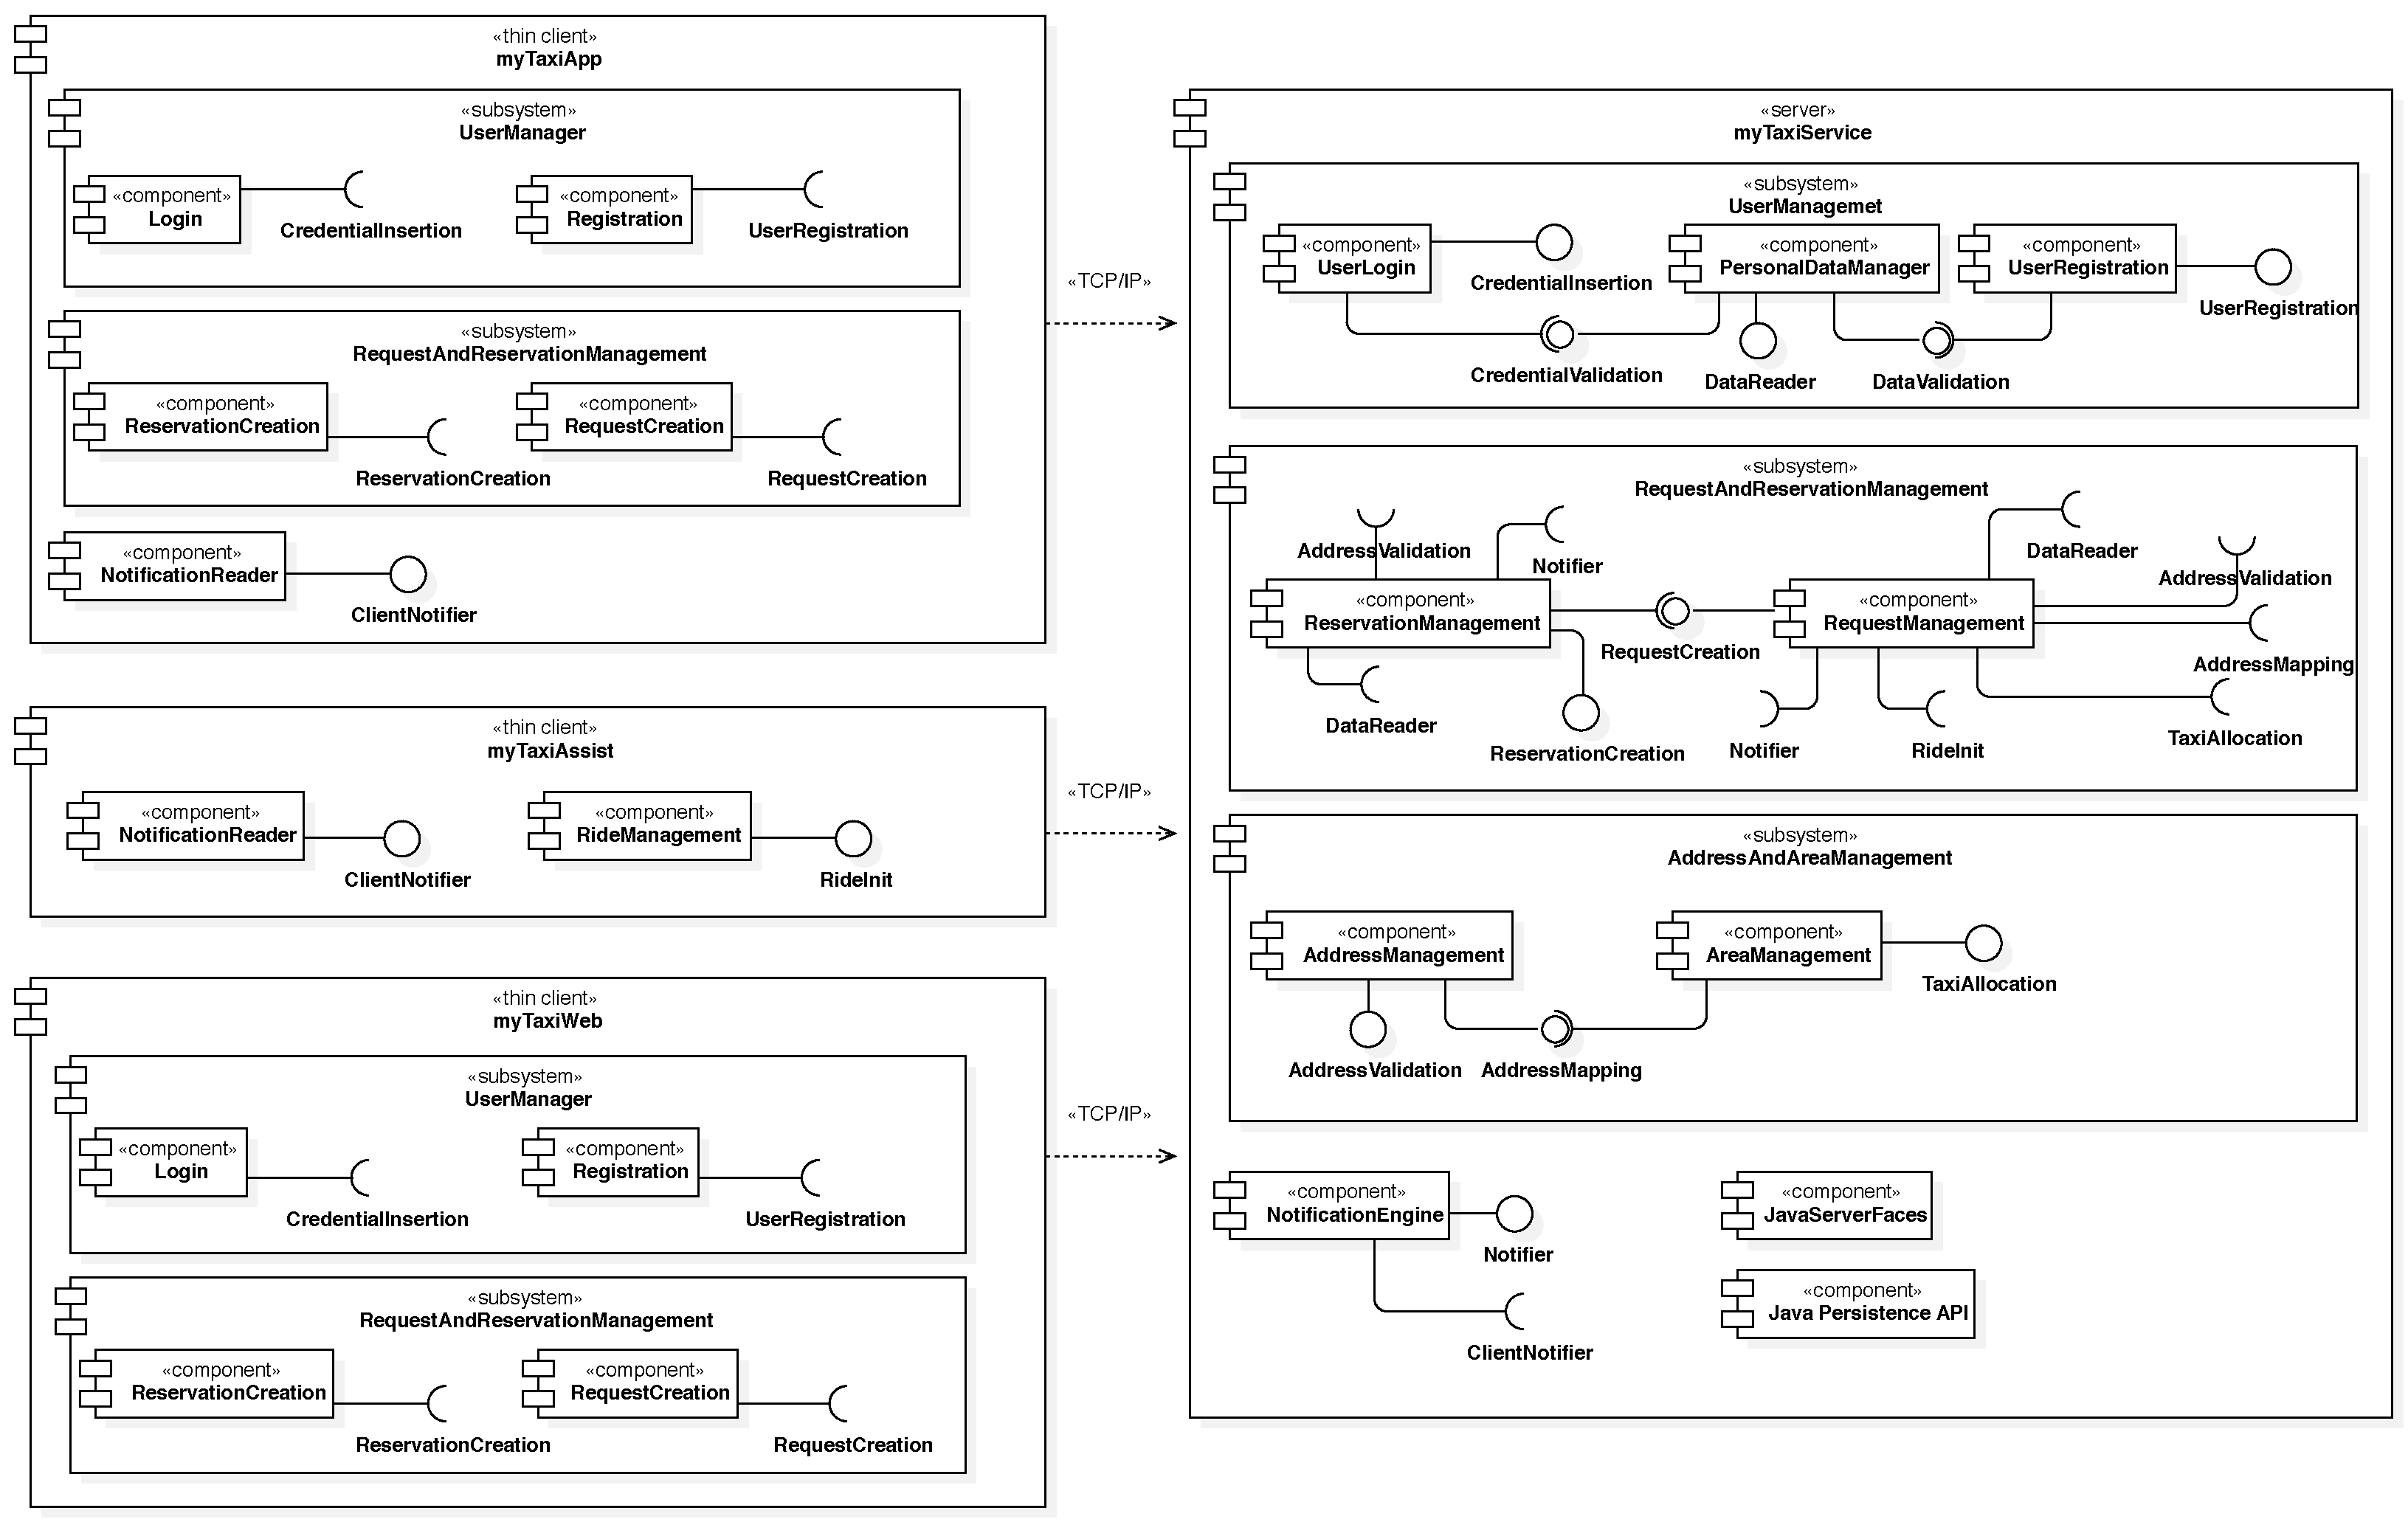
\includegraphics[width=\textwidth]{img/ComponentView__ComponentDiagram_1}%
	\caption{Component diagram.}%
	\label{fig:component}%
\end{figure*}

This testing plan covers most of the system. In particular, we are excluding \texttt{User\-Login} and \texttt{User\-Registration} components, as they would both need a comprehensive document on their own, as security protocols are needed. \texttt{Java\-Server\-Faces} and \texttt{Java Persistence API} are left out of this document, for the same reason.



\section{Integration testing strategy}
% Describe the integration testing approach (top down, bottom up, functional groupings, etc.) and the rationale for the choosing that approach.
As of the strategy to adopt in order to complete the integration test, we select the \mbox{top-down} approach. This way a verified input is going to be provided to the following component or subsystem to be integrated.

This incremental approach, focused on the architecture of the system, may require some additional work, since stubs need to be created extensively, but nevertheless should be easy to understand and arguably guarantee the quality of the software. At the end of the integration testing process, the fully functional system can be delivered to users, after undergoing a thorough system testing (which shall include also performance assessments and some evaluation about its behaviour under average and peak load).





\section{Integration sequence}
%NOTE: The structure of this section may vary depending on the integration strategy you select in Section 2.3. Use the structure proposed below as a non mandatory guide.
%\subsection{Software Integration Sequence} For each subsystem: Identify the sequence in which the software components will be integrated within the subsystem. Relate this sequence to any product features/functions that are being built up.
%\subsection{Subsystem Integration Sequence} Identify the order in which subsystems will be integrated.

%If you have a single subsystem, 2.4.1 and 2.4.2 are to be merged in a single section. You can refer to Section 2.2 of the test plan example [1] as an example of what we expect.



\begin{figure}%
	\centering%
	\includestandalone{img/sequence/sequence}%  
	\caption{Sequence of integration.}%
	\label{fig:intsequence}%
\end{figure}

















